\documentclass[a4paper, 11pt, titlepage]{jsarticle}
\usepackage[dvipdfmx]{graphicx}
\usepackage{listings}
\usepackage{amsmath}
\usepackage{url}
\usepackage{listings,jvlisting}
\lstset{
  basicstyle={\ttfamily},
  identifierstyle={\small},
  commentstyle={\smallitshape},
  keywordstyle={\small\bfseries},
  ndkeywordstyle={\small},
  stringstyle={\small\ttfamily},
  frame={tb},
  breaklines=true,
  columns=[l]{fullflexible},
  numbers=left,
  xrightmargin=0zw,
  xleftmargin=3zw,
  numberstyle={\scriptsize},
  stepnumber=1,
  numbersep=1zw,
  lineskip=-0.5ex
}

\title{知能情報実験III(データマイニング班)\\毒のある蛇かそうでないかを画像判別}
\author{215732C 佐久本元気\\215736F 西野大河\\215742A 米須悠\\215746C 新垣樹\\}
\date{提出日:2023年8月3日}
\begin{document}
\maketitle
\tableofcontents
\clearpage

\section{テーマ「毒のある蛇かそうでないかを画像判別」とは}
本グループでは画像で提示された蛇の毒の有無を予測することを対象問題として設定した。具体的な問題解決の方法としては、機械学習における画像認識・分類の技術を活用し、主にCNN(畳み込みニューラルネットワーク)を用いて行う。CNNは、\cite{theme1}によると「CNNはいくつもの深い層を持ったニューラルネットワークであり、主に画像認識の分野で価値を生んでいるネットワーク」で、「一般物体認識と呼ばれる画像認識のタスクで価値を発揮し、優れた性能を備えるアルゴリズム」とある。また、\cite{theme2}によると、「CNNの出力層はデータを解釈し、画像の予測や分類を行う」とある。
まとめると、CNNを用いることで蛇の画像の認識を行うことができ、蛇の毒の有無を予測することが可能であると考えられる。このテーマの実験を行うことの意義は、機械学習を用いた画像認識の仕方を学び、それらを様々なものに対する予測や分類に適用することができる点にあると考える。

\section{実験方法}
\subsection{実験目的・目標}
画像に写っている蛇の毒の有無を予測し、正しいか確認することが目的である。また、予測の正答率をできる限り高めることも目的の一つである。具体的な数値としては、正解率80\%を目標とする。

\subsection{データセット構築}
本実験では5種類のデータセットを構築して実験を行った。各データセットの名称は以下の通りである。\par
\begin{itemize}
\item classification snake species
\item Indian-Snakes-Dataset(以下 indian datasets と呼ぶ)
\item dataset1
\item dataset2
\item dataset3
\end{itemize}\par
なお、dataset1\textasciitilde3の画像収集にはGoogle Chromeの拡張機能である「Image downloader - Imageye」を利用した。\par

\clearpage

\subsection{前処理}
以下のようにして、機械学習モデルの正確性を上げた。

\subsubsection{データセットにおける前処理}
毎実験ごとに画像データを一枚一枚目でチェックし、クレンジングを行った。具体的には、他の動物が写っていたり、体の一部が欠けている蛇、アルビノなどノイズになりそうな画像などを各々分担しながら消去し、実験に用いた。

\subsubsection{データの正規化}
OpenCVで画像の前処理を行い、予測を適切に行えるようにした。具体的には、0\textasciitilde255の数字の集合である画像データを0\textasciitilde1の範囲に縮小することで、学習コストの削減を試みた。

\subsubsection{データ分割}
ホールドアウト法を用いて、以下のような割合でデータを分割した。\par
Train :70\%
Val:20\%
Test:10\%


\subsection{実験1}
\subsubsection{実験内容}
データセットをTrain, Val, Testで分割し、人がhappyかsadを識別する学習モデルを用いて、学習モデルの評価を行う。また、学習用としてKaggleで取得したデータセットのclassification snake speciesを利用する。\par

\subsubsection{モデル選定}
本実験では画像から毒あり毒無し蛇の特徴量を抽出してもらった上で予測を行うため、畳み込みやプーリングを行うことができるCNNをアルゴリズムとして採用した。
最後の出力としては0か1を出力させるのが目的なので、sigmoid関数を使う。\par
学習モデルの作成は、ImageClassification\cite{theme3}を参考に行なった。\par

\subsubsection{使用するデータセット}
Kaggle で取得したデータセットの classification snake species を利用する。\par
classification snake species (\url{https://www.kaggle.com/datasets/nikhilshingadiya/sample-0})

\subsubsection{パラメータ調整}
実験1ではパラメータを以下のように設定した。\par

\begin{lstlisting}[caption=パラメータ(実験1),label=fuga]
model = Sequential()
model.add(Conv2D(16, (3,3), 1, activation='relu', input_shape=(256,256,3))) 
#first layer needs to have input
model.add(MaxPooling2D())#take maximum value from 2x2 filter,only condence 

model.add(Conv2D(32, (3,3), 1, activation='relu'))
model.add(MaxPooling2D())

model.add(Conv2D(16, (3,3), 1, activation='relu'))
model.add(MaxPooling2D())

model.add(Flatten())#make it to 1D

#fully connected layers
#256neurons
model.add(Dense(256, activation='relu'))#going to have 256 values as our output
model.add(Dense(1, activation='sigmoid'))
#single output & map to 0 or1
\end{lstlisting}

以下はsummaryの結果である。\par
{\fontsize{10pt}{9pt}\selectfont
\begin{verbatim}
Model: "sequential"
_________________________________________________________________
 Layer (type)                Output Shape              Param #   
=================================================================
 conv2d (Conv2D)             (None, 254, 254, 16)      448       
                                                                 
 max_pooling2d (MaxPooling2  (None, 127, 127, 16)      0         
 D)                                                              
                                                                 
 conv2d_1 (Conv2D)           (None, 125, 125, 32)      4640      
                                                                 
 max_pooling2d_1 (MaxPoolin  (None, 62, 62, 32)        0         
 g2D)                                                            
                                                                 
 conv2d_2 (Conv2D)           (None, 60, 60, 16)        4624      
                                                                 
 max_pooling2d_2 (MaxPoolin  (None, 30, 30, 16)        0         
 g2D)                                                            
                                                                 
 flatten (Flatten)           (None, 14400)             0         
                                                                 
 dense (Dense)               (None, 256)               3686656   
                                                                 
 dense_1 (Dense)             (None, 1)                 257       
                                                                 
=================================================================
Total params: 3696625 (14.10 MB)
Trainable params: 3696625 (14.10 MB)
Non-trainable params: 0 (0.00 Byte)
_________________________________________________________________
\end{verbatim}
}


\subsection{実験2}
\subsubsection{実験内容}
学習済みモデルの作成および学習モデルの評価を行う。新たなデータセットdataset1を用いて学習し、上述のデータセットとは異なるindian datasetsを用いて再テストを行う。

\subsubsection{モデル選定}
実験1と同様にCNNを用いるが、すでに事前学習されているVGG16の全結合層以外のレイヤーにオリジナルでlayerを追加し、追加分レイヤーだけをファインチューニングして利用する。\par
オリジナルで追加したlayerの特徴としてはロバストネスのためのDropout layerを用いている。

\subsubsection{使用するデータセット}
訓練用データセット
\begin{itemize}
\item dataset1…無作為に選んだ毒蛇・毒なし蛇の画像(ハブやアカマタ等16種)を合計600枚程度集めたデータセット。
\end{itemize}\par
評価用データセット
\begin{itemize}
\item Indian-Snakes-Dataset(以下 indian datasetsと呼ぶ)…インドの毒蛇と毒なし蛇が含まれている信頼性の高いデータセット。GitHub上から、ダウンロードし利用する。\\
Indian-Snakes-Dataset  (\url{https://github.com/arjun921/Indian-Snakes-Dataset})
\end{itemize}

\subsubsection{パラメータ調整}
実験2ではパラメータを以下のように設定した。\par
\begin{lstlisting}[caption=パラメータ(実験2),label=fuga]
model = Sequential()

model.add(base_model)

model.add(Conv2D(64, kernel_size=3, padding="same", activation="relu"))
model.add(MaxPooling2D())
model.add(Dropout(0.25))

model.add(Flatten())
model.add(Dense(256, activation='relu'))
model.add(Dropout(0.5))
model.add(Dense(128, activation="relu")) 
model.add(Dense(64, activation="relu")) 
model.add(Dropout(0.5))

model.add(Dense(1, activation='sigmoid'))

\end{lstlisting}\par
以下はsummaryの結果である。\par
{\fontsize{10pt}{9pt}\selectfont
\begin{verbatim}
Model: "sequential_1"
_________________________________________________________________
 Layer (type)                Output Shape              Param #   
=================================================================
 vgg16 (Functional)          (None, 8, 8, 512)         14714688  
                                                                 
 conv2d_1 (Conv2D)           (None, 8, 8, 64)          294976    
                                                                 
 max_pooling2d_1 (MaxPoolin  (None, 4, 4, 64)          0         
 g2D)                                                            
                                                                 
 dropout_3 (Dropout)         (None, 4, 4, 64)          0         
                                                                 
 flatten_1 (Flatten)         (None, 1024)              0         
                                                                 
 dense_4 (Dense)             (None, 256)               262400    
                                                                 
 dropout_4 (Dropout)         (None, 256)               0         
                                                                 
 dense_5 (Dense)             (None, 128)               32896     
                                                                 
 dense_6 (Dense)             (None, 64)                8256      
                                                                 
 dropout_5 (Dropout)         (None, 64)                0         
                                                                 
 dense_7 (Dense)             (None, 1)                 65        
                                                                 
=================================================================
Total params: 15313281 (58.42 MB)
Trainable params: 598593 (2.28 MB)
Non-trainable params: 14714688 (56.13 MB)
_________________________________________________________________
\end{verbatim}
}\par
実験の際には、VGG16の全結合層以外のレイヤーを用い、その下にlayerを追加した。
これらの重みに関しては、VGG16モデルの重みをImageNetデータセットから事前に学習されたものに設定された状態のままにしておくため、これの重みは更新しないこととする。
オリジナルで追加したlayerにのみ重みを更新することとする。

\subsection{実験3}
\subsubsection{実験内容}
実験2で作成した学習済みモデルを利用し、同様に学習モデルの評価を行う。新たなデータセットdataset2を用いて学習し、indian datasetsを用いて精査を行う。

\subsubsection{モデル選定}
実験2で用いた学習モデルをそのまま使用する。

\subsubsection{使用するデータセット}
訓練用データセット
\begin{itemize}
\item dataset2…実験2で訓練用データセットとして用いたdataset1に世界各地の毒蛇、毒なし蛇の画像を追加したデータセット。地域を北アメリカ州、南アメリカ州、アフリカ州、ヨーロッパ州、アジア州(さらに東南アジア、南アジア、中央アジア、西アジアに分ける)、オセアニア州に分け、各地域ごとに毒蛇、毒なし蛇を各2\textasciitilde5種類選定する。その中から地域ごとの蛇の画像が合計5枚になるようにデータセットに追加した。
\end{itemize}\par
評価用データセット
\begin{itemize}
\item indian datasets …実験2同様のデータセット。
\end{itemize}

\subsubsection{パラメータ調整}
実験2と同様に行う。

\subsection{実験4}
\subsubsection{実験内容}
実験2で作成した学習済みモデルを利用し、同様に学習モデルの評価を行う。新たなデータセットdataset3を用いて学習し、indian datasetsを用いて精査を行う。

\subsubsection{モデル選定}
実験2で用いた学習モデルをそのまま使用する。

\subsubsection{使用するデータセット}
訓練用データセット
\begin{itemize}
\item dataset3…実験3で訓練用データセットとして用いたdataset2に各地域ごとの蛇の画像をさらに追加したデータセット。追加した枚数の内訳は以下の通りである。
\end{itemize}\par

\clearpage

\begin{table}[htb]
\centering
  \caption{データセット3に追加した枚数の内訳}
  \begin{tabular}{|c|c|c|}  \hline
    地域 & 毒あり & 毒なし \\ \hline \hline
    北アメリカ州 & 96 & 120 \\ \hline
    南アメリカ州 & 135 & 60 \\ \hline
    アフリカ州 & 143 & 80 \\ \hline
    ヨーロッパ州 & 148 & 100 \\ \hline
    東南アジア & 89 & 60 \\ \hline
    南アジア & 143 & 180 \\ \hline
    中央アジア & 54 & 30 \\ \hline
    西アジア & 61 & 90 \\ \hline
    オセアニア州 & 91 & 30 \\ \hline \hline
    合計 & 960 & 750 \\ \hline
  \end{tabular}
\end{table}

評価用データセット
\begin{itemize}
\item indian datasets …実験2同様のデータセット。
\end{itemize}

\subsubsection{パラメータ調整}
実験2と同様に行う。

\section{実験結果}
各実験における学習モデルの評価や精査の結果は以下の通りになった。ここで実験結果として示されている数値として、性能評価指標(適合率・再現率・正解率)がある。適合率は、正確に予想された陽性サンプル数/予測された陽性サンプル数で表される。再現率は、正確に予測された陽性サンプル数/実際の陽性サンプル数で表される。正解率は、(正確に予測された陽性サンプル数+正確に予測された陰性サンプル数)/全サンプル数で表される。
\subsection{実験1}

\clearpage

\begin{figure}[htbp]
  \begin{minipage}[b]{0.45\linewidth}
    \centering
    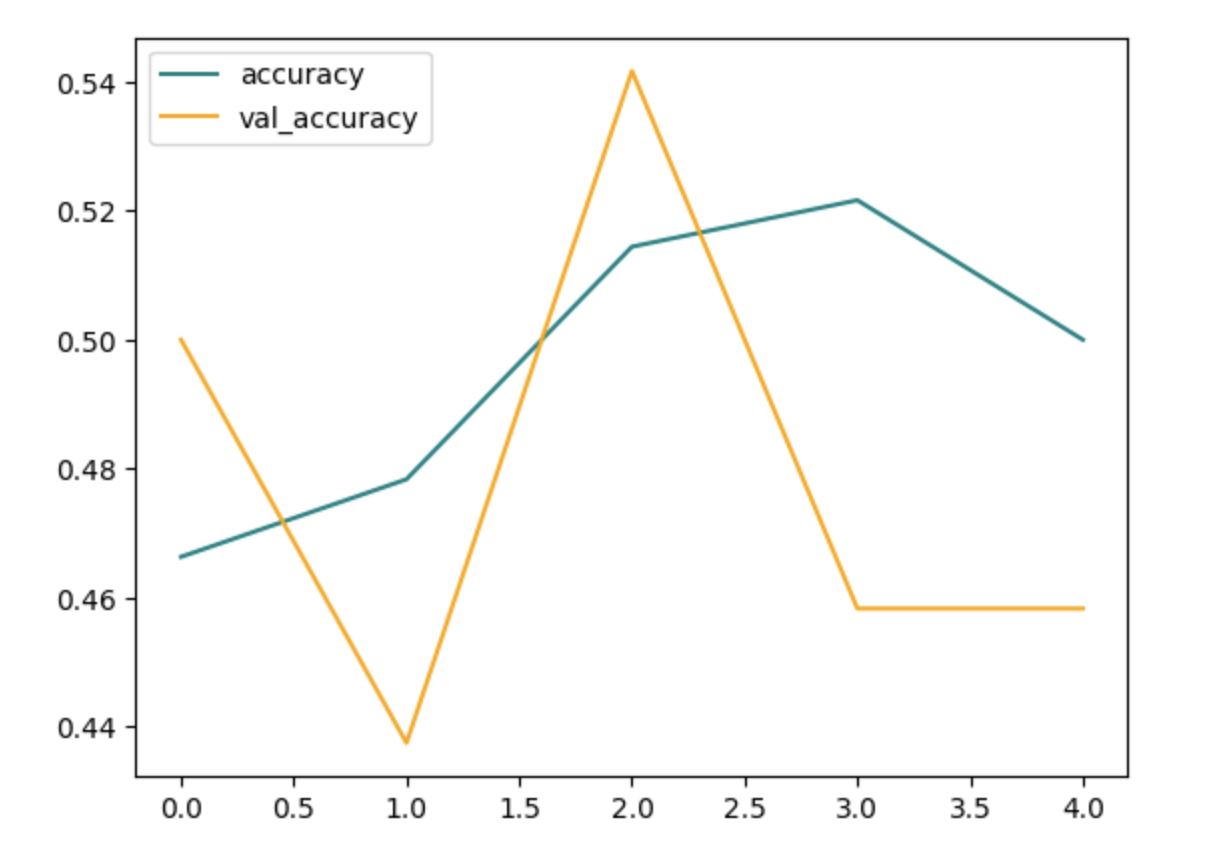
\includegraphics[keepaspectratio, scale=0.32]{ex1_acc.png}
    \caption{実験1 Accuracy}
  \end{minipage}
  \begin{minipage}[b]{0.45\linewidth}
    \centering
    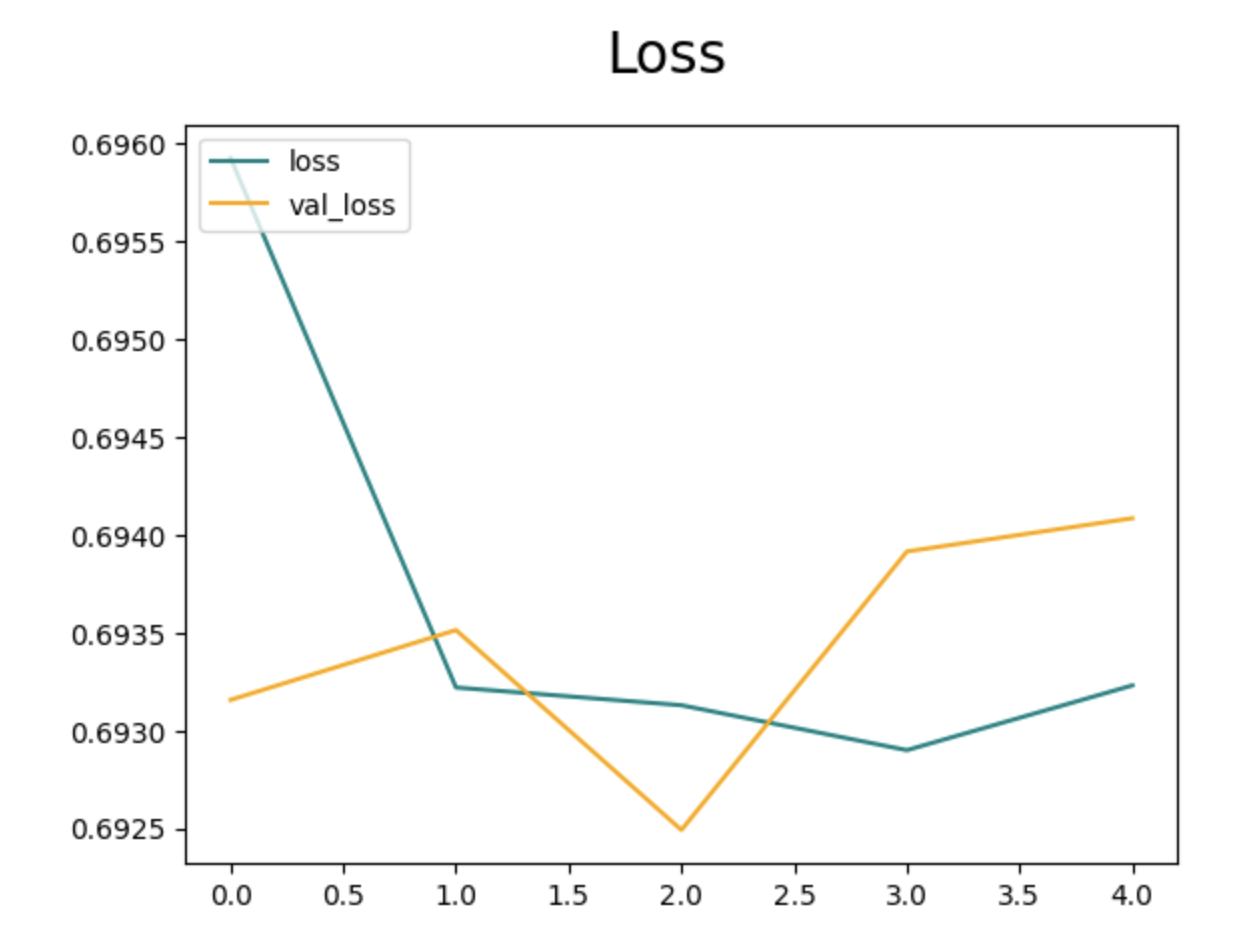
\includegraphics[keepaspectratio, scale=0.32]{ex1_loss.png}
    \caption{実験1 Loss}
  \end{minipage}
\end{figure}

\subsubsection{学習モデルの評価}

\begin{itemize}
\item 適合率:tf.Tensor(0.453125, shape=(), dtype=float32)
\item 再現率:tf.Tensor(1.0, shape=(), dtype=float32) 
\item 全体の正解率:tf.Tensor(0.453125, shape=(), dtype=float32)
\end{itemize}


\subsection{実験2}
\begin{figure}[htbp]
  \begin{minipage}[b]{0.45\linewidth}
    \centering
    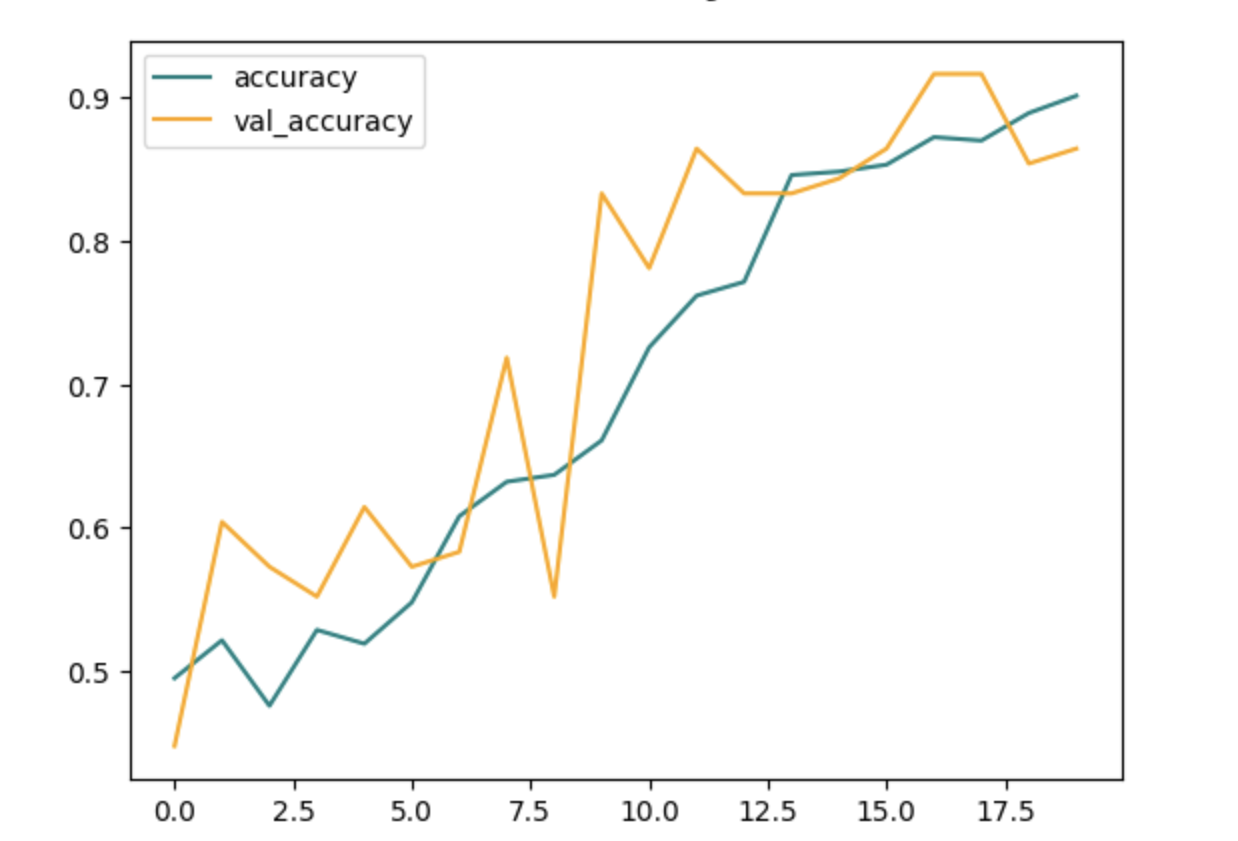
\includegraphics[keepaspectratio, scale=0.33]{ex2_acc.png}
    \caption{実験2 Accuracy}
  \end{minipage}
  \begin{minipage}[b]{0.45\linewidth}
    \centering
    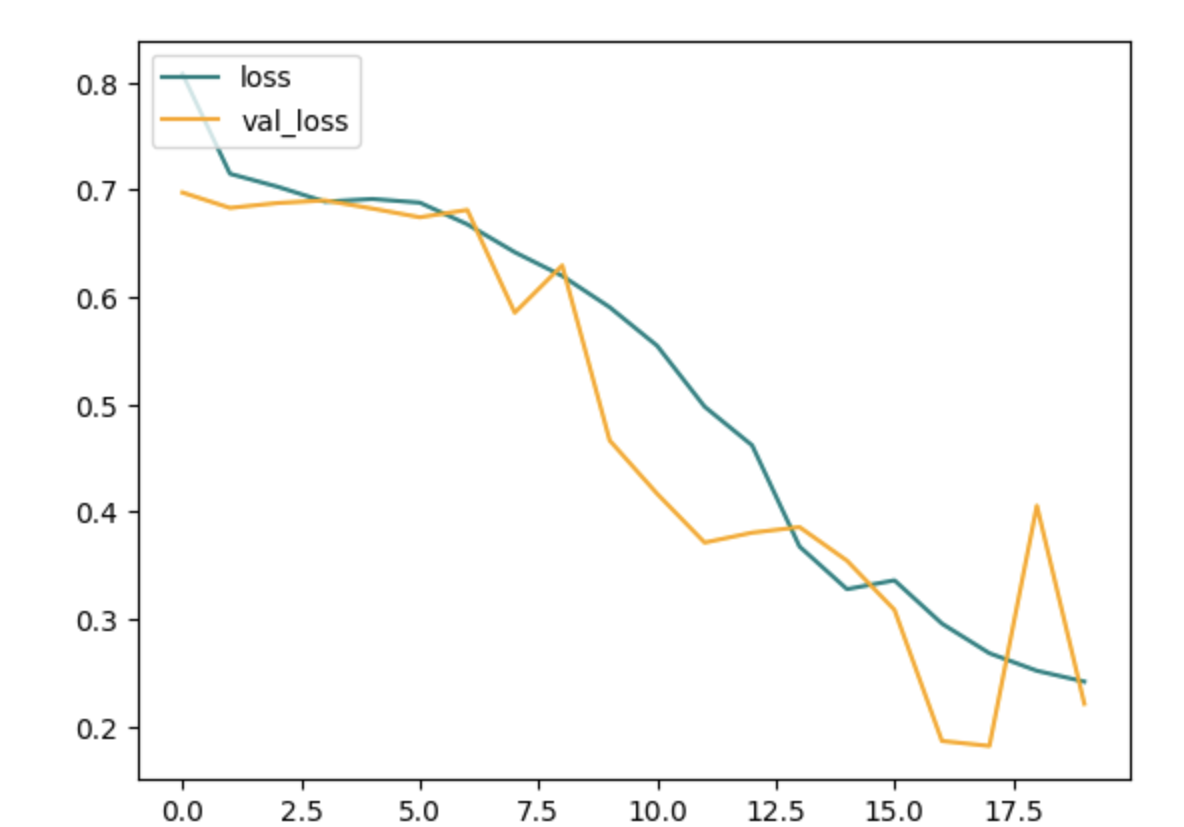
\includegraphics[keepaspectratio, scale=0.33]{ex2_loss.png}
    \caption{実験2 Loss}
  \end{minipage}
\end{figure}

\subsubsection{学習モデルの評価}
\begin{itemize}
\item 適合率:tf.Tensor(0.96638656, shape=(), dtype=float32)
\item 再現率:tf.Tensor(0.7615894, shape=(), dtype=float32) 
\item 正解率:tf.Tensor(0.8566308, shape=(), dtype=float32)
\end{itemize}
\subsubsection{indian datasetsによる精査}
\begin{itemize}
\item 適合率:tf.Tensor(0.6117647, shape=(), dtype=float32)
\item 再現率:tf.Tensor(0.3939394, shape=(), dtype=float32) 
\item 正解率:tf.Tensor(0.44607842, shape=(), dtype=float32)
\end{itemize}

\subsection{実験3}
\begin{figure}[htbp]
  \begin{minipage}[b]{0.45\linewidth}
    \centering
    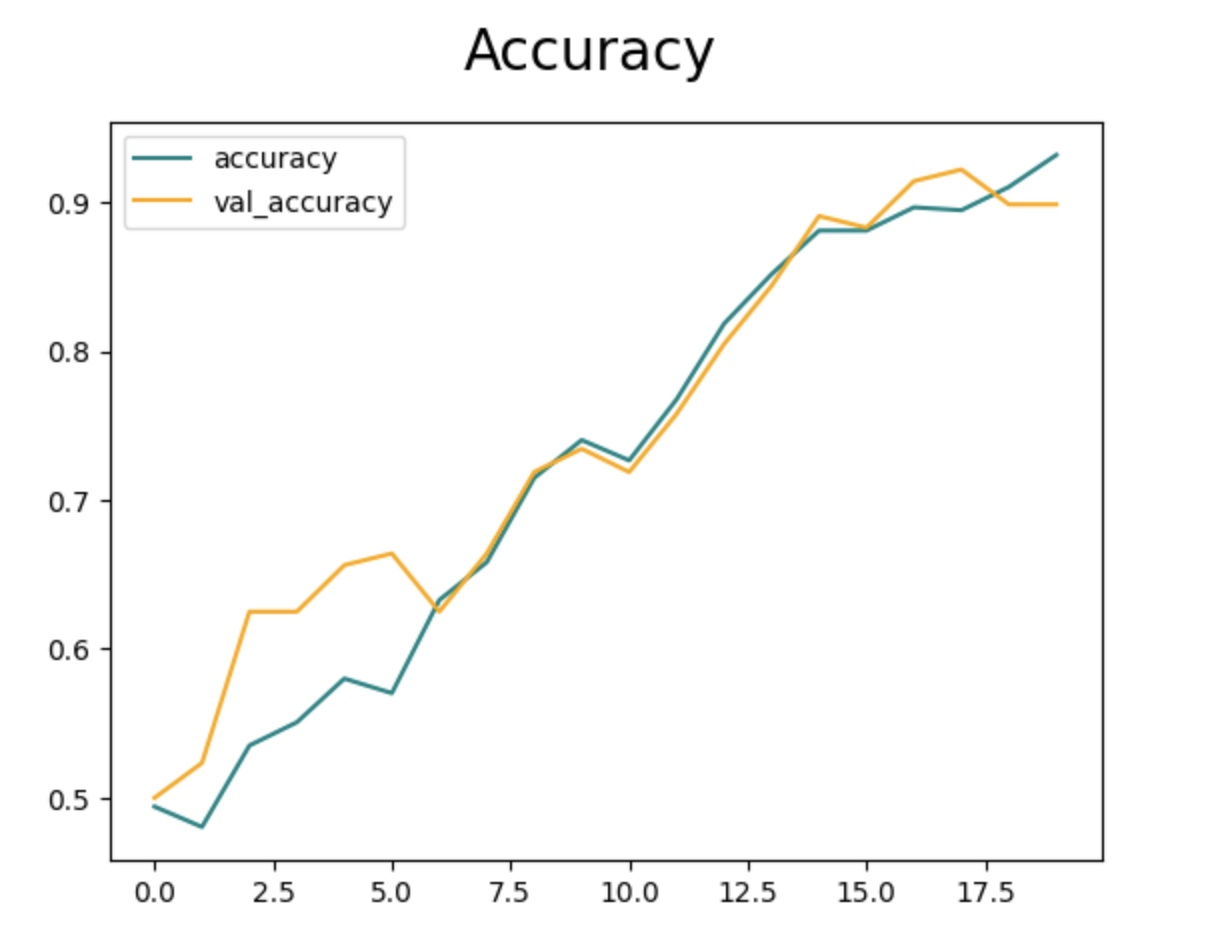
\includegraphics[keepaspectratio, scale=0.161]{ex3_acc.jpg}
    \caption{実験3 Accuracy}
  \end{minipage}
  \begin{minipage}[b]{0.45\linewidth}
    \centering
    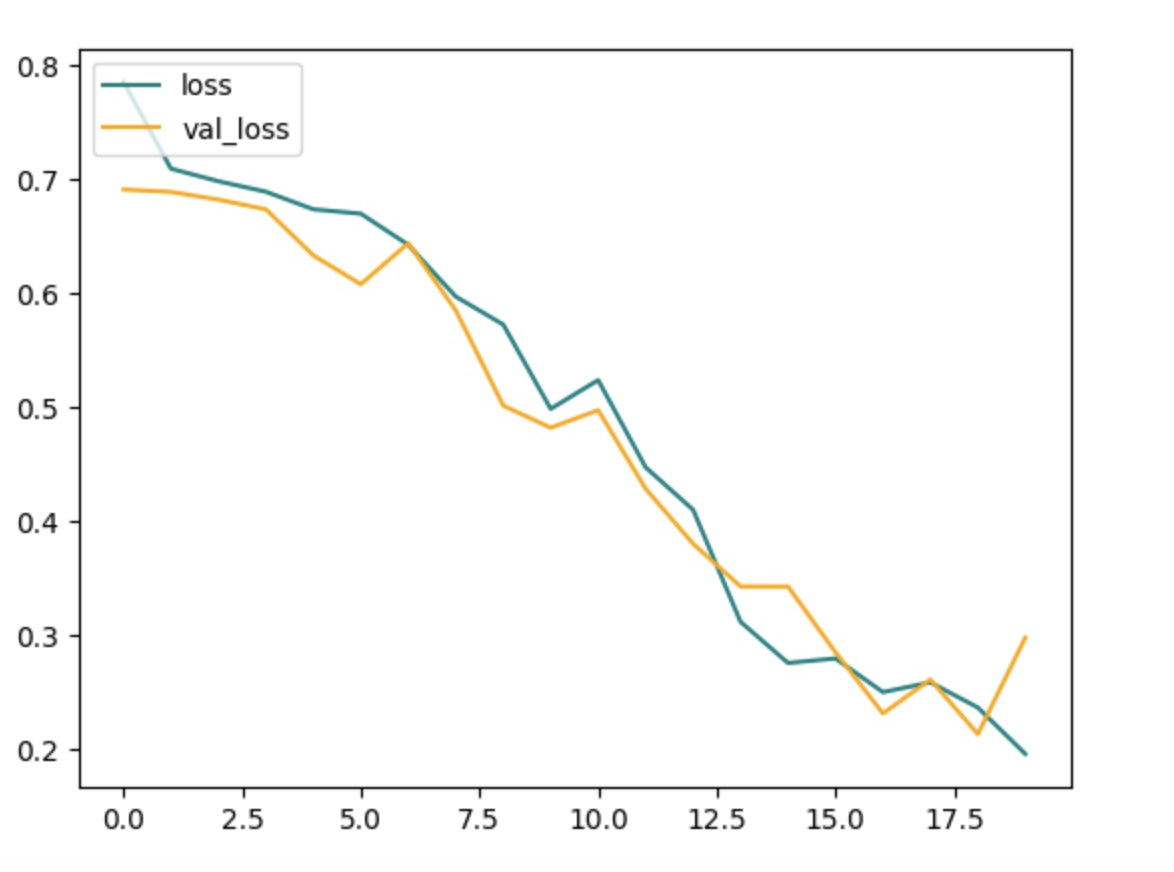
\includegraphics[keepaspectratio, scale=0.161]{ex3_loss.jpg}
    \caption{実験3 Loss}
  \end{minipage}
\end{figure}

\subsubsection{学習モデルの評価}
\begin{itemize}
\item 適合率:tf.Tensor(0.972973, shape=(), dtype=float32)
\item 再現率:tf.Tensor(0.8181818, shape=(), dtype=float32) 
\item 正解率:tf.Tensor(0.9052632, shape=(), dtype=float32)
\end{itemize}
\subsubsection{indian datasetsによる精査}
\begin{itemize}
\item 適合率:tf.Tensor(0.7126437, shape=(), dtype=float32)
\item 再現率:tf.Tensor(0.5344828, shape=(), dtype=float32) 
\item 正解率:tf.Tensor(0.5611111, shape=(), dtype=float32)
\end{itemize}

\clearpage

\subsection{実験4}
\begin{figure}[htbp]
  \begin{minipage}[b]{0.45\linewidth}
    \centering
    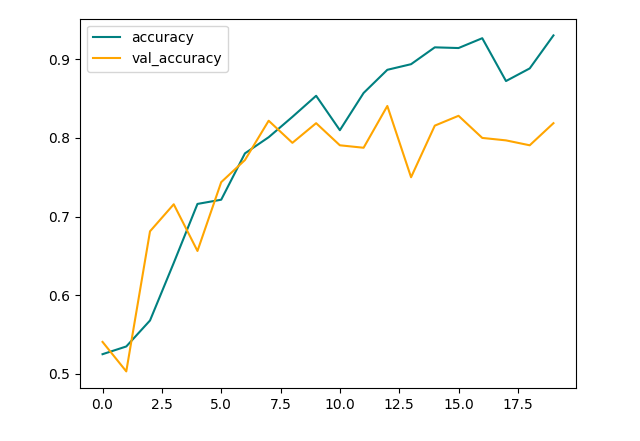
\includegraphics[keepaspectratio, scale=0.435]{ex4_acc.png}
    \caption{実験4 Accuracy}
  \end{minipage}
  \begin{minipage}[b]{0.45\linewidth}
    \centering
    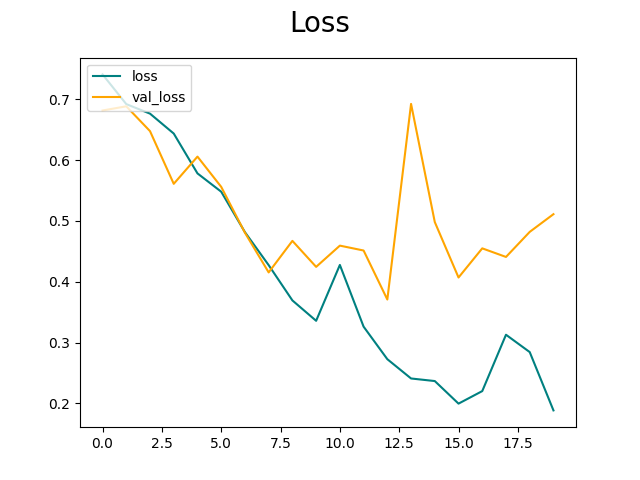
\includegraphics[keepaspectratio, scale=0.435]{ex4_loss.png}
    \caption{実験4 Loss}
  \end{minipage}
\end{figure}

\subsubsection{学習モデルの評価}
\begin{itemize}
\item 適合率:Precision result: 0.8222222328186035
\item 再現率:Recall result: 0.9367088675498962
\item 正解率:Binary Accuracy result: 0.8432835936546326
\end{itemize}
\subsubsection{indian datasetsによる精査}
\begin{itemize}
\item 適合率:Precision result: 0.699999988079071
\item 再現率:Recall result: 0.6968609690666199
\item 正解率:Binary Accuracy result: 0.6092020869255066
\end{itemize}

\section{考察}
\subsection{実験1}
うまくいかなかった原因として、データセットと学習モデル両方に問題があったと考えられる。データセットは、kaggleで取得したデータセットを利用したが、体の一部が無い絶命状態の蛇や、人間の写真など投稿者のプライベート画像が大量に混入しており、信頼性のないものであった。学習モデルは、学習反復回数が5回のみで非常に少なかったことが挙げられる。また、過学習対策を行わなかったことも原因の一つとして挙げられる。他にも、蛇の画像を識別するのに、人間の表情を見分ける学習モデルを用いたことも原因として挙げられる。\par
実験1から学んだ改善点として、データセットに関しては、より適切なデータセットを探した上で、データのクレンジングを行うことが挙げられる。また、毒蛇と無毒蛇を種類ごとに調べることで、データセットの正確性を高められると考えた。学習に関しては、学習回数が足りてないように感じたため、学習反復回数を5回から20回に増やすことが挙げられた。また、VGG16のような汎用的な学習済みモデルにファインチューニングを施すことや、過学習による汎化性能の低下の対策として、NNモデルにdropout layerを追加することが挙げられた。\par

\subsection{実験2}
実験2で用いた訓練用データセットの蛇の種類は、主に日本の蛇が中心だったため、indian datasetsの特徴量と合致していなかったと考えられる。元々、毒蛇共通の特徴があると仮定して実験を行なっていたが、どちらにせよ外国の蛇のデータは必要だと考えた。\par
また、今回用いたデータセットに世界各国の毒蛇と無毒蛇の画像をそれぞれ追加することが必要だと考えた。膨大な種類の画像が必要になるため、今後の開発ではデータセットを作成する人員を増やして実験を進めていくべきだと考えられる。

\subsection{実験3}
画像を追加したデータセットの内容は一種ごとで10倍の差があっため、外国の蛇に対する特徴量は導きにくいと予想した。一方、精査結果のスコアが向上していたため、さらにデータセットを充実させれば目標に達する可能性があると考えられる。\par
そこで、データセットに追加する分の画像を蛇一種あたり30枚ほどに増加させることで、正解率向上を目指せるのではないかと考えた。なお、追加する蛇の種類はすでに確定しており、実験2での画像追加より作業量は多くならないと見込まれるため、データセットを作成する人員を減らして進める。

\subsection{実験4}
うまくいかなかった原因として、Train,Val,Testデータにそれぞれデータの偏りがあったことが挙げられる。また、データセットの画像が多すぎたことから、ノイズを完全に取り除けていなかった可能性があった。\par
改善点として、交差検証を行うことが挙げられる。本実験は、ホールドアウト法で行なっていたため、データの偏りを考慮していなかった。また、説明変数を減らして汎化性能を高めるために、正則化の実装が挙げられる。\cite{theme4}

\clearpage

\section{意図していた実験計画との違い}
行った実験の流れをガントチャートを用いて、表すと以下の通りになった。\par
\begin{figure}[htbp]
\begin{center}
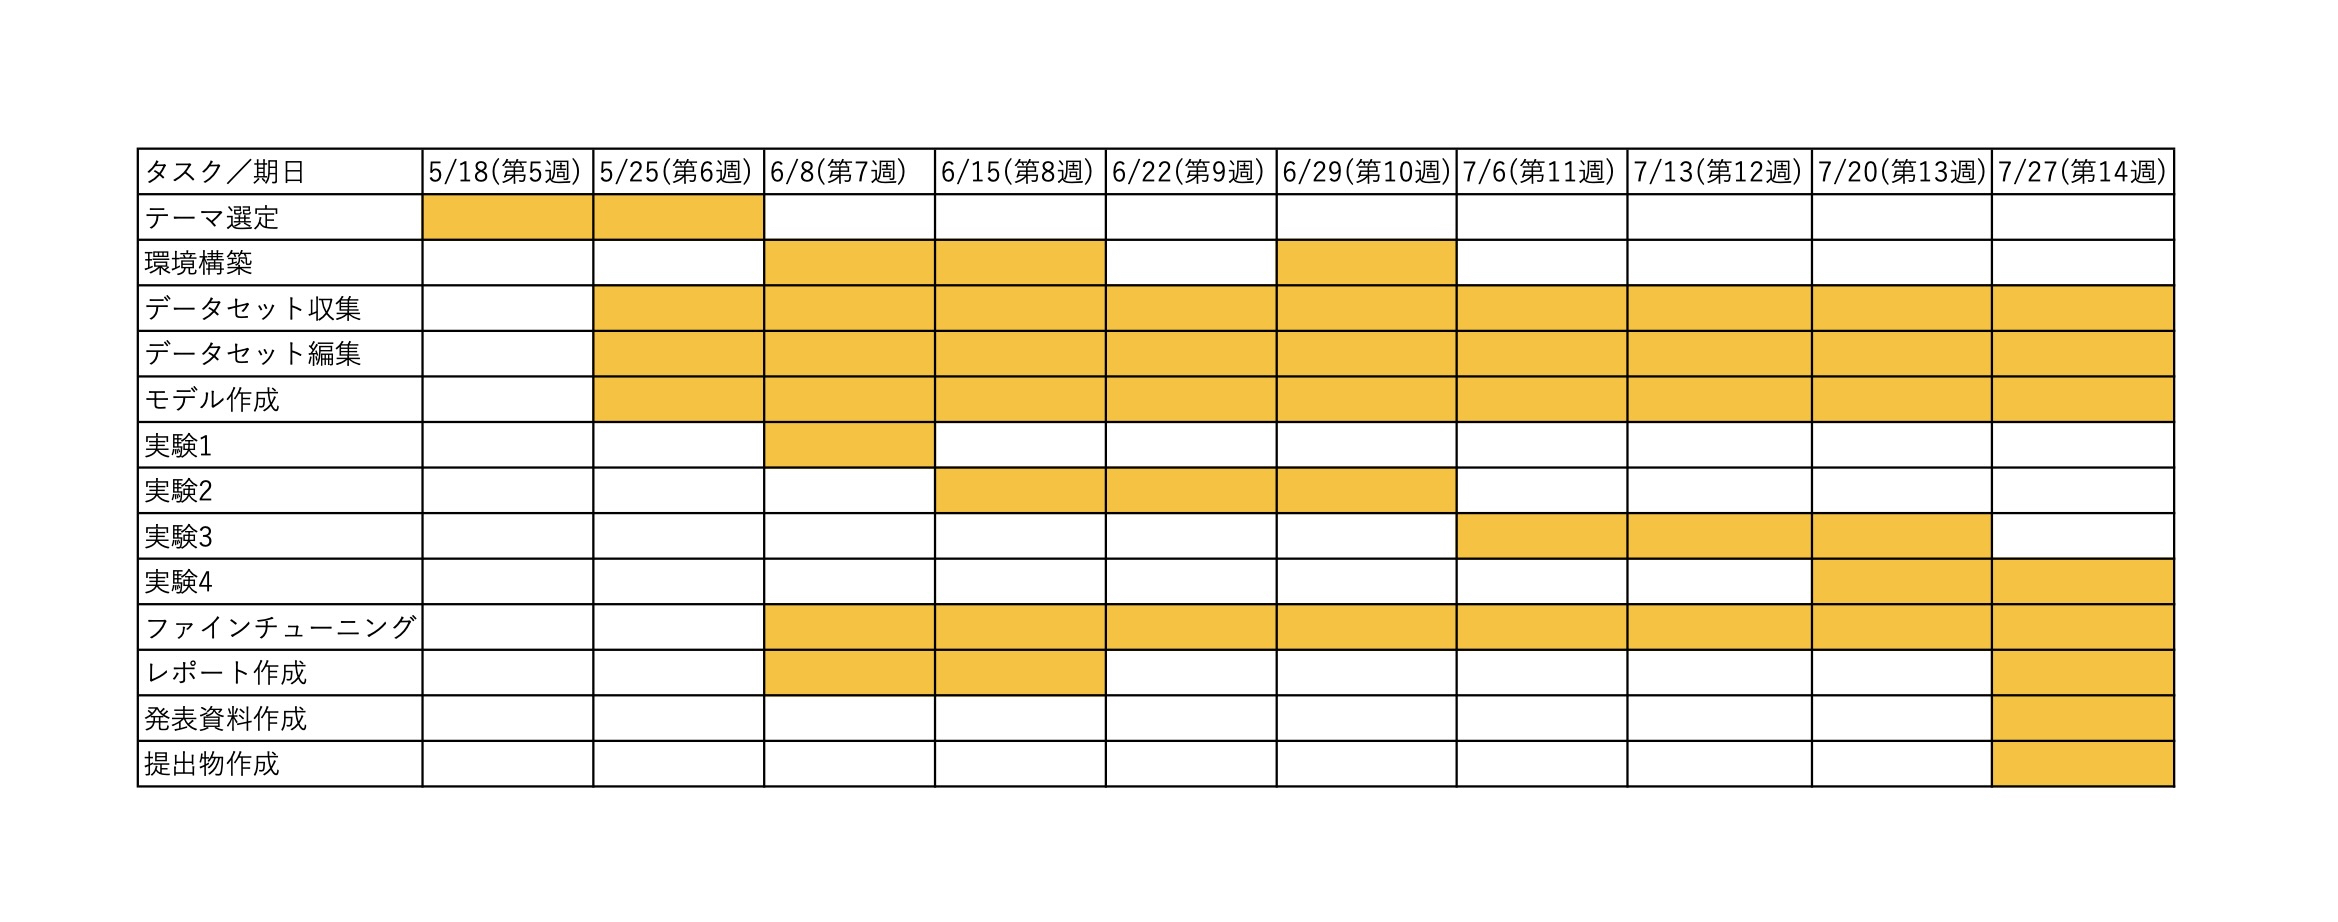
\includegraphics[width=150mm]{G2_Ganttchart.jpeg}
\caption{実験の流れ}
\end{center}
\end{figure}
想定していた以上に環境構築で躓いてしまい、本来1週で構築する予定だったが3週ほどかかってしまった。データセットに関しては、開発期間全体を通して収集・編集をおこない、正答率向上を目指した。

\section{まとめ}
今回の実験では、画像に写っている蛇の毒の有無を予測し、正しいか確認することを目的として、正解率80\%を目指して実施した。残念ながら、最終的な正解率は約60\%と目標を達成することができなかった。しかし、実験の中で気づいた点として、「データセットの充実性」についての重要性が挙げられる。データセットをテスト用のデータに対応させるために工夫するたび、正解率が上がっていったことから、機械学習におけるデータセット内容の重要性について再認識することができた。また、実験を進めていくにつれ、機械学習の手法や開発に対する取り組み方についての理解を深めることができた。他にもGitHubを利用したバージョン管理や学科サーバーを利用した実験なども行うことができ、チーム開発として良い点だったと考える。

\begin{thebibliography}{n}
	\bibitem{theme1}画像認識でよく聞く「CNN」とは?仕組みや特徴を1から解説, \url{https://aismiley.co.jp/ai_news/cnn/}, 2023/06/14.
	\bibitem{theme2}画像認識の分野では欠かせない「CNN(畳み込みネットワーク)とは」, \url{https://www.paloaltoinsight.com/2022/12/09/cnn/},2023/06/14.
	\bibitem{theme3}ImageClassification, \url{https://github.com/nicknochnack/ImageClassification}, 2023/06/08
	\bibitem{theme4}NRI 野村総合研究所 用語解説 過学習\url{https://www.nri.com/jp/knowledge/glossary/lst/ka/overfitting},2023/08/03
\end{thebibliography}
\end{document}
